\documentclass[12pt]{article}
\usepackage{epsfig}
\usepackage{color}
\usepackage{graphicx}
\usepackage{amssymb,amsmath}
\usepackage{wrapfig}
\usepackage{amsmath}
\usepackage{amssymb}


\definecolor{orange}{cmyk}{0,0.4,0.8,0.2}
\definecolor{darkorange}{rgb}{.71,0.21,0.01}
\definecolor{darkgreen}{rgb}{.12,.54,.11}
\definecolor{darkblue}{rgb}{0.1,0.1,0.8}
\usepackage{hyperref}
\hypersetup{pdftex,  % needed for pdflatex
  breaklinks=true,  % so long urls are correctly broken across lines
  colorlinks=true,
  urlcolor=blue,
  linkcolor=darkorange,
  citecolor=darkgreen,
  }

\pagestyle{plain}
\topmargin 0in
\headheight 0in
\headsep 0in
\footskip 0.5in

\textheight 9.0in
\textwidth 6.5in

\oddsidemargin 0in
\evensidemargin 0in
\marginparwidth 0in
\baselineskip0.2cm
\parskip0.1cm
\font\cap=cmcsc10

\def\ni{\noindent}        %No Indent%
\def\ub{\underbar}
\def\hi{\noindent \hangindent=2.5em}
\def\et{{\it et\thinspace al.}}    %et al.%
\def\hour{^{\rm h}}
\def\minute{^{\rm m}}
\def\second{^{\rm s}}
\def\arcmin{^{\prime}}
\def\arcsec{^{\prime\prime}}
\def\pixel{{\rm\,pixel}}
\def\degrees{{\rm\,degrees}}
\def\pc{{\rm\,pc}}
\def\cm{{\rm\,cm}}
\def\kms{{\rm\,km/s}}
\def\kpc{{\rm\,kpc}}
\def\hkpc{{\rm\,$h_{50}^{-1}$\,kpc}}
\def\hpc{{\rm\,$h_{50}^{-1}$\,pc}}
\def\Mpc{{\rm\,Mpc}}
\def\mpc{{\rm\,Mpc}}
\def\Gyr{{\rm\,Gyr}}
\def\kmsec{{\rm\,km/s}}
\def\hnot{{\rm\,km/s/Mpc}}
\def\msun{{\rm\,M_\odot}}
\def\lsun{{\rm\,L_\odot}}
\def\mdot{{\rm\,M_\odot}}
\def\surfb{{\rm\,mag/arcsec^2}}
\def\araa{{\it Ann.\ Rev.\ Astr.\ Ap.}}
\def\actaa{{\it Acta~Astronomica}}
\def\aj{{\it A.~J.}}  %Astronomical Journal%
\def\apj{{\it Ap.~J.}}  %Astrophysical Journal%
\def\apjs{{\it Ap.~J.~Suppl.}}  %Astrophysical Journal Supplements%
\def\apjl{{\it Ap.~J.~(Letters)}} %Astrophysical Journal Letters%
\def\pasp{{\it Pub.~A.S.P.}}      %Publications of the Astronomical%
                                %Society of the Pacific%
\def\memsai{{\it Memorie della Societ� Astronomica Italiana}}
\def\mn{{\it M.N.R.A.S.}}      %Monthly Notices of the Royal%
                                %Astronomical Society%
\def\mnras{{\it M.N.R.A.S.}}      %Monthly Notices of the Royal%
                                %Astronomical Society%
\def\nat{{\it Nature}}      %Nature%
\def\aa{{\it Astr.~Ap.}}     %Astronomy & Astrophysics%
\def\aap{{\it Astr.~Ap.}}     %Astronomy & Astrophysics%
\def\aasup{{\it Astr.~Ap.~Suppl.}}     %A & A Supplements%
\def\aaps{{\it Astr.~Ap.~Suppl.}}     %A & A Supplements%
\def\ass{{\it Astr.~Sp.~Sci.}}     %A & A Supplements%
\def\an{Astronomische~Nachrichten}%
\def\MW{Milky Way }

%
% \lta and \gta produce > and < signs with twiddle underneath
%
\def\spose#1{\hbox to 0pt{#1\hss}}
\def\lta{\mathrel{\spose{\lower 3pt\hbox{$\mathchar"218$}}
     \raise 2.0pt\hbox{$\mathchar"13C$}}}
\def\gta{\mathrel{\spose{\lower 3pt\hbox{$\mathchar"218$}}
     \raise 2.0pt\hbox{$\mathchar"13E$}}}

% also mine!
\def\gsim{\,\lower3pt\hbox{$\sim$}\llap{\raise2pt\hbox{$>$}}\,}
\def\lsim{\,\lower3pt\hbox{$\sim$}\llap{\raise2pt\hbox{$<$}}\,}

% marina
\newcommand{\beqas}{\begin{eqnarray*}}
\newcommand{\eeqas}{\end{eqnarray*}}
\newcommand{\beqa}{\begin{eqnarray}}
\newcommand{\eeqa}{\end{eqnarray}}
\newcommand{\xdelta}{\ensuremath{x^\Delta}}
\newcommand{\comment}[1]{}

\def\xdeltax#1{\ensuremath{x^{\Delta #1}}}
\def\Lo{\hbox{$L_{\odot}$}}
\def\Mo{\hbox{$M_{\odot}$}}

\newcommand{\epss}{\ensuremath{\varepsilon}}
\newcommand{\epsz}{\ensuremath{\varepsilon^0}}
\newcommand{\epstild}{\ensuremath{\tilde{\varepsilon}}}
\newcommand{\psf}{\ensuremath{P\!S\!F\!}}
\newcommand{\SN}{S\!N}
\newcommand{\VS}{V\!S}
\newcommand{\KBO}{K\!B\!O\!}

\newlength{\boxwidth}
\newlength{\boxdown}
\newlength{\boxheight}

\renewcommand{\contentsname}{Table of Contents}
\pagenumbering{gobble}
\begin{document}
\begin{center}
\LARGE{Astronomy: \\Cosmic Ideas and\\Our Gateways to\\the Universe}\\
\vspace{2in}
\Large{\today}\\
\vspace{2in}
\Large{Nicholas Hunt-Walker\\Harlem Children's Zone - Summer 2014}
\end{center}
\vfill
\break

% Table of Contents - 
\tableofcontents
\vfill
\break

%  Skeleton Outline and Objective
\pagenumbering{arabic}
\setcounter{page}{1}
\addcontentsline{toc}{part}{\hspace {1em}Motivation and Curriculum Outline}
\section*{Motivation}

Young kids---particularly those of middle school age---are naturally awed by and enthusiastic about the sciences because science is their first real introduction into how the world works. These fresh concepts spark their imagination of what is and isn't possible in the Universe. However, as they get older they encounter a combination of dry, formulaic teaching and a lack of connection to the real world which stifles the imagination and causes interest in the sciences to crumble. This imagination is essential to experiencing the benefits of science. The damaging effects are that much more severe, where there is the societal expectation that people of color aren't cut out for science, a field dominated by people that don't look, act, or think like them. Their lack of a desire to be in that unimaginative, unengaging, and unfamiliar environment manifests in mew forms in their minds. Many conclude that science, as a whole, is boring and therefore they never aspire to develop the ability to understand science at all.\\

As a student I have experienced classroom models and teaching styles that deter students and some that engage students. For three years I have served as a teaching assistant at the college and high school levels. I have been looking for opportunities to improve my presentation in an environment of my own creation.  I realize that the Harlem Children's Zone services a large demographic of students of color. I am particularly interested in working with youngsters from the Harlem Children's Zone because I have personally witnessed a severely low presence of minorities in the hard sciences.  As such, I have designed this course to counteract disillusionment in those critical middle-school years. My curriculum does not skimp on content or rigor that is necessary to truly understand the cosmos. For six weeks I will lead my students on a fun-filled, intriguing journey through the various objects that occupy our Universe. We will tour the concepts of the night sky, and cover some of the landmark technologies that brought us knowledge of the Universe and allow the students to make their own discoveries of what is in the Universe that surrounds us. Ultimately, I want students to feel that same interest in the science of the Universe as they felt when they first saw the stars.\\





\vfill
\break

%  Skeleton Outline and Objective
\addcontentsline{toc}{part}{\hspace {1em}Curriculum Outline}
\section*{Curriculum Outline}
\begin{itemize}
\item Elective
\item \textbf{Time:} \\50 minutes per class; 3 days per week; 1 or 2 groups per day (depending on interest).
\item \textbf{Capacity:} \\20 students maximum per class.
\item \textbf{Format and Activities:} \\ Interacting with Microsoft's WorldWide Telescope software (I maintain our University's version of the software, so there's no learning curve for me), various hands-on or interactive activities, dedicated class-long labs, chalkboard lectures, and PowerPoint lectures. I will incorporate daily take-home challenges where students will be required to solve problems, conduct their own investigations and create their own scientific data record-keeping system. 
\item \textbf{Assignments:} \\Classwork daily, homework twice per week, lab assignments over the weekends.
\item \textbf{Integrated Subjects:} \\
	The benefits of scientific study---particularly astronomy---inherently provides for the intermingling of various subjects:
	\begin{itemize}
	\item Mathematics (algebra, geometry, arithmetic, trigonometry)
	\item Physics (gravity, motion, energy, light, sound)
	\item Geology (rock types, rock dating, volcanoes, earthquakes)
	\item Chemistry (basic reactions, atmospheric gases, phases of matter)
	\item Biology (photosynthesis, DNA, eyes, water in the body)
	\end{itemize}
	
\item \textbf{Expected Outcomes:}
	\begin{itemize}
	\item Students will obtain a new or renewed appreciation for the wonders of science
	\item Students will learn how to apply basic and intermediate mathematics to practical situations
	\item Students will become familiar with the logical and integrative thought processes inherent in the Scientific Method
	\item Students will realize that humans are not omniscient and will accept the fact that questions should be asked. They will feel comfortable pursuing unknown knowledge
	\item Students will become comfortable expressing and testing their ideas
	\end{itemize}


\end{itemize}
\subsection*{Week 1 - Basic Physics and the Moon}
\begin{itemize}
\item Day 1: Pictures of the sky, gravity, object motion
	\begin{itemize}
	\item \textbf{Demonstration}: Magnetic accelerator cannon
	\item \textbf{Activity}: Build a catapult and predict where it shoots
	\end{itemize}
\item Day 2: The Moon, its origins, and its age
	\begin{itemize}
	\item \textbf{Activity}: Age dating rocks from radioactive decay
	\end{itemize}
\item Day 3: More on the Moon, it's dynamic history, building a simple telescope
	\begin{itemize}
	\item \textbf{Lab}: Build a simple reflecting telescope and look at the Moon's craters.
	\end{itemize}
\end{itemize}

\subsection*{Week 2 - Planet Formation, More on Gravity, Intro to Light}
\begin{itemize}
\item Day 1: What is a planet and how is it formed?
	\begin{itemize}
	\item \textbf{Activity}: Create a planet with its own plants and animals, atmosphere, day/year length.
	\end{itemize}
\item Day 2: How planets settle into orbits around stars, and predicting planet orbits
	\begin{itemize}
	\item \textbf{Activity}: Build a star system
	\end{itemize}
\item Day 3: Finding other planets
	\begin{itemize}
	\item \textbf{Lab}: Detecting planets with radial velocities and transits
	\end{itemize}
\end{itemize}

\subsection*{Week 3 - Life of the Sun and Much About Light}
\begin{itemize}
\item Day 1: Formation and life of the Sun
	\begin{itemize}
	\item \textbf{Activity}: Gas pressure vs elasticity showing hydrostatic equilibrium.
	\end{itemize}
\item Day 2: The Sun's light carries energy and tells us about it's composition
	\begin{itemize}
	\item \textbf{Demo}: Radiometer
	\item \textbf{Demo}: Light through a prism
	\item \textbf{Demo}: Different colors of fire and spectra
	\end{itemize}
\item Day 3: The Sun's light interacts with matter and creates all our sky color and sunsets.
	\begin{itemize}
	\item \textbf{Demo}: Shining light through a cloudy tank of water
	\item \textbf{Lab}: Solving a Light Maze
	\end{itemize}
\end{itemize}

\subsection*{Week 4 - Other Stars and Space Travel}
\begin{itemize}
\item Day 1: Wide variety of stars and their deaths
	\begin{itemize}
	\item \textbf{Demo}: Relative sizes of stars in the galaxy
	\end{itemize}
\item Day 2: Rockets and space travel
	\begin{itemize}
	\item \textbf{Outing/Lab}: Hike to Central Park.  Students build their own rockets to the stars
	\end{itemize}
\item Day 3: The truth and world history behind the constellations
	\begin{itemize}
	\item \textbf{Activity}: Create your own constellation and constellation story
	\end{itemize}
\end{itemize}

\subsection*{Week 5 - The Milky Way Galaxy and Other Galaxies}
\begin{itemize}
\item Day 1: The Milky Way in our sky and its contents in different wavelengths
	\begin{itemize}
	\item \textbf{Demo}: Views of the sky with WorldWide Telescope
	\end{itemize}
\item Day 2: \textbf{Field Trip}: Columbia University Department of Astronomy

\item Day 3: Other Galaxies 
	\begin{itemize}
	\item \textbf{Demo}: Wide variety of other galaxies and classifications
	\item \textbf{Lab}: Form a galaxy
	\end{itemize}
\end{itemize}

\subsection*{Week 6 - The Rest of the Cosmos}
\begin{itemize}
\item Day 1: Dark Matter \& Dark Energy
	\begin{itemize}
	\item \textbf{Demo}: Gravitational lensing
	\end{itemize}
\item Day 2: The Big Bang and evolution of the Cosmos
	\begin{itemize}
	\item \textbf{Lab}: Inflate a Universe
	\end{itemize}
\item Day 3: \textbf{Field Trip}: American Museum of Natural History Hayden Planetarium 

\end{itemize}

\vfill
\break

% Body of Proposal
\addcontentsline{toc}{part}{\hspace{1em}Curriculum Description}
\section*{Curriculum Description}
Astronomy is the study of the night sky, the Universe, and ultimately ourselves. Through astronomy we seek to answer questions of our origins, the motions of the universe, and the objects that twinkle in the dark. This course is a detailed walk through the science and technologies of the field, revealing to students the objects and concepts that have occupied the greatest human minds for centuries.\\

We begin with a brief description of the science of astronomy. I'll describe how astronomy grew from  simply tracking the stars in the sky to the science of their study. Then we'll move to the most prominent object in the night sky: the Moon. We'll discuss its dynamic history and growth into what we see today. We'll discuss its violent formation, dynamic life, and then learn to find its age.  We'll see the truth behind its phases, and connect that to what we see in the night sky throughout each month. We'll then build our own telescopes and survey its surface with our own eyes.\\

Our next stop is planets in and out of our Solar System. We'll learn what makes a planet, then how a planet is made. Some of the most advanced technology today is dedicated to finding planets, so we'll talk about those technologies as well as practice their planet-finding method. As humans, our main concern is how planets either allow for or discourage life. As such, we focus in on all the necessary components that allow life as we know it, including how planets maintain (and lose) atmospheres.\\

From there we have a natural transition to the fire in our sky, the Sun. We'll open the door to the furnace of its interior learning about what nuclear fusion is and how it works. It's constantly in a battle with itself between expansion and wholesale collapse, and we'll see how that happens. Then we'll learn how its life will end, and what that means for our planet. The Sun gives our planet all of its life, light, and energy. In fact, light is the most important thing in astronomy. It's how we know most of what we do about the Universe. As such, we'll see what light is, how it works, and learn to harness and manipulate it ourselves.\\

Our Sun is only one of the hundreds of billions of stars within our galaxy. The events of their lives characterize our night sky, and we'll discuss how each type of star lives. We will also come to see what makes stars are red, yellow, or blue (and why none are green!). We'll talk about space travel to those stars and what makes it so difficult. Then we'll build simple compressed-water rockets to mimic those that got all of our satellites into space, and will one day get astronauts to other stars. Having learned all about the stars in our sky, we'll use them to create our own constellations and stories to match.\\
%http://workshop.chromeexperiments.com/stars/

We see each star individually, but the ensemble of all of the stars in our sky are part of what constitutes our Galaxy. We will learn about the other components of our galaxy (gas, dust, etc.), and discuss its overall structure. Galaxies don't live static lives, so we'll see how nearby galaxies influence one another and give us the myriad of shapes and structures that we see in space.\\
%http://mcdonaldobservatory.org/teachers/classroom/MakeYourOwnGalaxy.html

The last stop on our journey will zoom out to our Universe as a whole. We'll discuss what we believe to be its origins, and talk about the dark mysteries that continue to elude astronomers today. We will even create our own mini universes, and learn about how their expansion illustrates what we see in our own universe. Then we head to the American Museum of Natural History for more activities, details on class topics, and a planetarium show about our dark universe.\\

Learning happens best when there is work being done inside and outside of the classroom. As such, in addition to the activities, labs, and demonstrations, I will send students home with a short question set about each week's topic, as well as encourage them to ask me questions about space, specifics of different space missions, or careers in astronomy and astrophysics. Lastly, because the beauty of the cosmos is what draws all eyes toward the night sky, I will have students search through the archives of Astronomy Picture of the Day (\url{http://apod.nasa.gov/apod/astropix.html}) each week and come up with an image that interests them, with an explanation of their interest. Through six weeks of these lessons and assignments, students will be sure to walk away with a deeper understanding of the science and contents of our night sky.


\vfill
\break

% Brief Bio
\addcontentsline{toc}{part}{\hspace{1em}Career Biography}
\title{Nicholas Hunt-Walker Brief Career Biography}
\maketitle

\begin{wrapfigure}{l}{0.225\textwidth}
\vspace{-15pt}
%\begin{center}
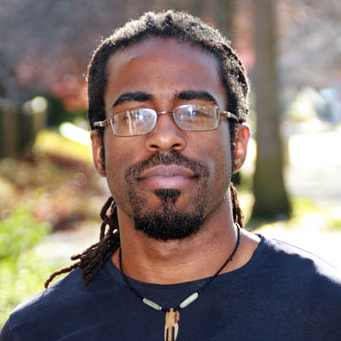
\includegraphics[width=0.2\textwidth]{profile.jpg}
%\end{center}
\vspace{-10pt}
\end{wrapfigure}
\noindent Nicholas discovered his love for physics during his junior and senior years of high school at Elmont Memorial Junior-Senior High School. This continued at the City University of New York (CUNY) at Queensborough Community College when he took his first course in astronomy. This course caused him to change from a major in business administration and transfer to CUNY York College in 2007 to pursue his Bachelor's degree in physics and mathematics. After two and a half years at York, he finished his undergraduate career with the Post-Baccalaureate Program at Columbia University, serving as a researcher in high-energy astrophysics.  In the late summer of 2010 he moved to Seattle, where he began his graduate studies in astronomy at the University of Washington (UW). He has thus far obtained his Masters of Science in astronomy (2012), and is currently in pursuit of his Ph.D.\\

Throughout his journey from Queensborough to UW, Nicholas has been fortunate to have been given many opportunities to learn be a researcher, a presenter, as well as a teacher. In the summer of 2006, his astronomy professor at Queensborough enabled him to perform research looking into solar activity leading up to solar flares, despite not having a major in physics or astronomy. He also tutored for the College Discovery program for a year, assisting students in account, mathematics, and astronomy. While at York College, he was fortunate to take part in a number of research projects in both physics and astronomy. He worked in a lab investigating the properties of water in elastic tissue using Nuclear Magnetic Resonance probes. In the summer 2007 he interned at the Smithsonian Institute's National Air and Space Museum. The summer of 2008 brought him to the American Museum of Natural History as a participant of the National Science Foundation's Research Experiences for Undergraduates (NSF-REU) program. While there, he studied the rate of star formation in distant galaxies. The following summer, he participated in another NSF-REU at the University of Wisconsin, studying exotic X-ray sources in nearby dwarf galaxies. During the year that followed he delved heavily into gamma-ray astronomy on two projects, searching for gamma-ray emission from a distant galaxy with one, and looking for high-energy stellar remnants with another. All the while, he tutored physics, mathematics, and chemistry for freshmen and sophomores at York College. Currently, he is searching for clues to the structure of our own Milky Way galaxy for his Ph.D. thesis, while spending his sixth academic quarter as a teaching assistant for freshmen astronomy classes. 


\vfill
\break

% Budget Needs
\addcontentsline{toc}{part}{\hspace{1em}Materials and Budget}
\section*{Materials and Budget}
\begin{center}
\begin{figure}[h]
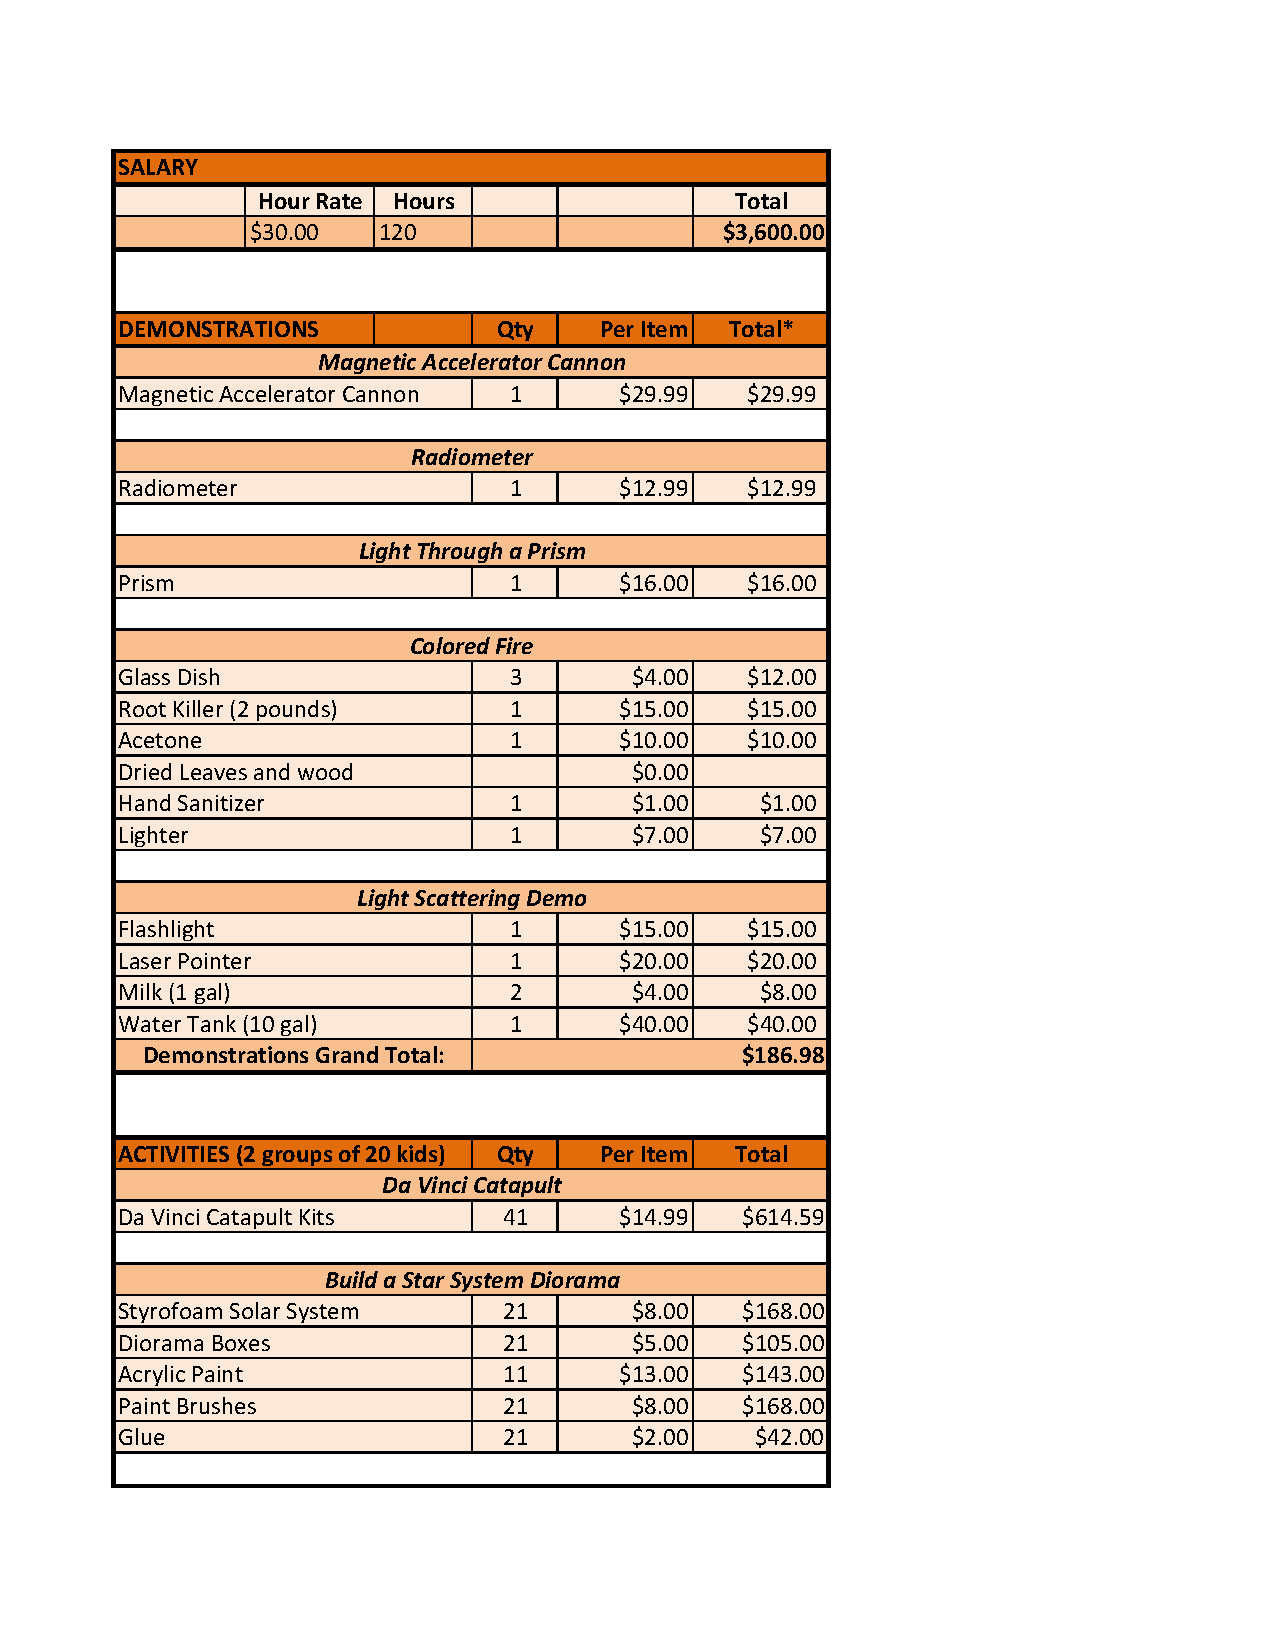
\includegraphics[width=4in,height=7in]{budget1.pdf}
\end{figure}
\end{center}

\begin{center}
\begin{figure}[h]
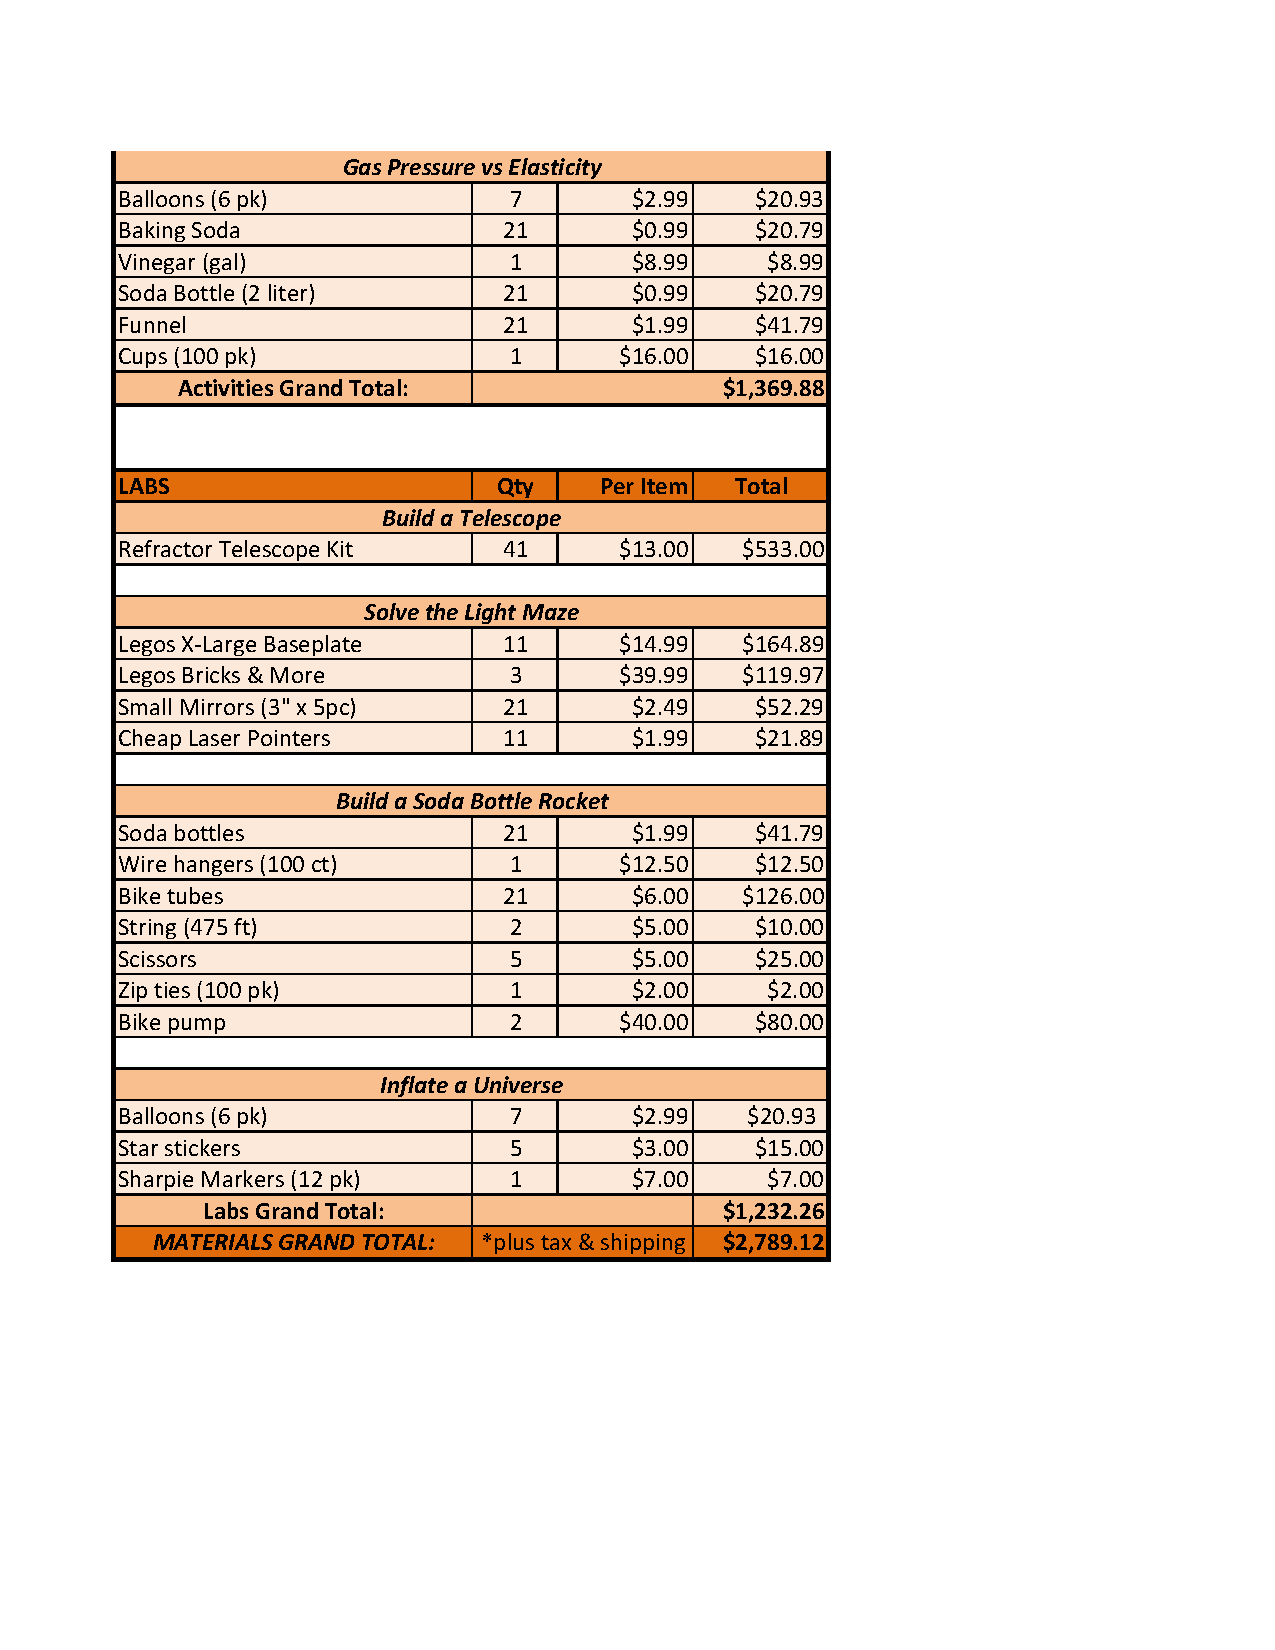
\includegraphics[width=4in]{budget2.pdf}
\end{figure}
\end{center}

\vfill
\break




\end{document}